%%%%%%%%%%%%%%%%%%%%%%%%%%%%%%%%%%%%%%%%%
% Stylish Article
% LaTeX Template
% Version 2.1 (1/10/15)
%
% This template has been downloaded from:
% http://www.LaTeXTemplates.com
%
% Original author:
% Mathias Legrand (legrand.mathias@gmail.com) 
% With extensive modifications by:
% Vel (vel@latextemplates.com)
%
% License:
% CC BY-NC-SA 3.0 (http://creativecommons.org/licenses/by-nc-sa/3.0/)
%
%%%%%%%%%%%%%%%%%%%%%%%%%%%%%%%%%%%%%%%%%

%----------------------------------------------------------------------------------------
%	PACKAGES AND OTHER DOCUMENT CONFIGURATIONS
%----------------------------------------------------------------------------------------

\documentclass[fleqn,10pt]{SelfArx} % Document font size and equations flushed left

\usepackage[brazil]{babel} % Specify a different language here - english by default

\usepackage{lipsum} % Required to insert dummy text. To be removed otherwise

% Modificações

\usepackage{amsmath} % necessario para muitas funções nas equações

\usepackage{siunitx} % para uniforam numeros e unidades no arquivo

\usepackage[numbers]{natbib} % bibliografia moderna

% \usepackage{url}

% IMAGENS

\graphicspath{{./images/}} % configurar a pasta de imagens

% IMPORTANTE

% Se trabalhar com BIBLATEX, usar nas configurações do compilador a ordem: PDFLATEX --> BIBTEX --> PDFLATEX --> PDFLATEX
% Em TeXstudio: Options --> Configure TeXstudio --> Build --> Default compiler: txs:///pdflatex | txs:///bibtex | txs:///pdflatex | txs:///pdflatex

%----------------------------------------------------------------------------------------
%	COLUMNS
%----------------------------------------------------------------------------------------

\setlength{\columnsep}{0.55cm} % Distance between the two columns of text
\setlength{\fboxrule}{0.75pt} % Width of the border around the abstract

%----------------------------------------------------------------------------------------
%	COLORS
%----------------------------------------------------------------------------------------

\definecolor{color1}{RGB}{0,0,90} % Color of the article title and sections
\definecolor{color2}{RGB}{0,20,20} % Color of the boxes behind the abstract and headings

%----------------------------------------------------------------------------------------
%	HYPERLINKS
%----------------------------------------------------------------------------------------

\usepackage{hyperref} % Required for hyperlinks
\hypersetup{hidelinks,colorlinks,breaklinks=true,urlcolor=color2,citecolor=color1,linkcolor=color1,bookmarksopen=false,pdftitle={Title},pdfauthor={Author}}

\usepackage[anythingbreaks]{breakurl}  % Necessario para quebrar URLS na bibliografia
\def\UrlBreaks{\do\/\do-}

%----------------------------------------------------------------------------------------
%	ARTICLE INFORMATION
%----------------------------------------------------------------------------------------

\JournalInfo{COQ897 Otimização de Processos} % Journal information
\Archive{Prof. Argimiro Secchi} % Additional notes (e.g. copyright, DOI, review/research article)

\PaperTitle{Otimização Dinâmica da Produção de Anticorpos Monoclonais em Células Animais} % Article title

\Authors{Jasper Hendrik Moltrecht} % Authors
\affiliation{\textsuperscript{1}\textit{Universidade Federal do Rio de Janeiro/UFRJ, Chemical Engineering Program/COPPE, Rio de Janeiro, RJ, Brazil}} % Author affiliation
\affiliation{*\textbf{Corresponding author}: jasper@peq.coppe.ufrj.br} % Corresponding author

\Keywords{Otimização Dinâmica --- Cultura de Células Animais --- Anticorpos Monoclonais} % Keywords - if you don't want any simply remove all the text between the curly brackets
\newcommand{\keywordname}{Palavras-Chave} % Defines the keywords heading name

%----------------------------------------------------------------------------------------
%	ABSTRACT
%----------------------------------------------------------------------------------------

\Abstract{A indústria biofarmacêutica fornece produtos farmacêuticos baseados em proteínas com valor elevado, produzidos por células microbianas e animais. A cultura de células animais é o único método para produzir proteínas com modificações pós-translacionais idênticos com os do humano, que são aplicados a um amplo conjunto de doenças. Porém, pela complexidade do metabolismo das células e restrições das agências reguladoras, o processo de cultivo indica investimentos elevados, ambos no financiamento e na mão de obra. A otimização dos processos é tradicionalmente feita apenas por estudos experimentais, no entanto há maior interesse em métodos que envolvem abordagens computacionais. Modelos adequados e validados proporcionam valoroso conhecimento sobre o processo, e em cima disso permitem estudos de otimização ou controle ótimo. Nesse estudo, a modelagem de distintos modos de operação de biorreatores em taque agitato foi realizada. Em cima disso, diferentes aplicações da otimização dinâmica foram esboçados, começando com determinação da melhor estratégia de alimentação na batelada alimentada, da melhor taxa de diluição na operação continua e controle ótimo na perfusão.}
	
	
%	a controle ótima de em processo de produção de anticorpos monoclonais em batelada alimentada foi determinada, tendo a vazão de alimentação como variável de controle e maximização da concentração de anticorpos como função de objetivo. Os resultados indicam que uma estratégia de alimentação ótima pode aumentar o título de anticorpos por até  \SI{20}{\percent} em comparação com culturas não-otimizadas.}

%----------------------------------------------------------------------------------------

\begin{document}

\flushbottom % Makes all text pages the same height

\maketitle % Print the title and abstract box

\tableofcontents % Print the contents section

\thispagestyle{empty} % Removes page numbering from the first page

%----------------------------------------------------------------------------------------
%	ARTICLE CONTENTS
%----------------------------------------------------------------------------------------

\section*{Introdução} % The \section*{} command stops section numbering

\addcontentsline{toc}{section}{Introdução} % Adds this section to the table of contents

A industria de bioprocessos é responsável pela produção de uma grande quantidade de agentes terapêuticos e diagnósticos de origem biológica. A maioridade desses produtos são drogas baseadas em proteínas (como anticorpos, hormônios e fatores de crescimento) e são destinados a aplicações terapêuticas ou para uso como ferramentas de diagnóstico \textit{in vivo}. Os anticorpos monoclonais (mAbs) constituem a classe de proteínas terapêuticas mais estudada e utilizada atualmente, aprovados para o tratamento de uma variedade de doenças como câncer, esclerose múltipla ou desordens autoimunes, que afeitam a qualidade de vida de milhões de pessoas \cite{Bettinardi2016,Koumpouras2012}.

Em 2013, biofármacos geraram receitas globais de US\$ 163 bilhões, que é por volta de \SI{20}{\%} do mercado farmacêutico. O setor das biofármacos está crescendo a taxas anuais maior que \SI{8}{\%}, o dobro do setor de fármacos em geral. Entre os 10 biofármacos mais vendidos no mundo, sete são mAbs e derivados, os quais corresponderam a \SI{54,2}[US\$~] bilhões em 2013 \cite{otto2014,Walsh2014}. 

No brasil, a maioria das biofármacos tem que ser importados, e geram uma economia de R\$ \num{4.1} bilhões por ano nas compras públicas, que é mais que a metade (\SI{51}{\%}) dos gastos do Ministério da Saúde. No entanto, o estabelecimento de uma produção própria de biosimilares\footnote{Medicamento biofarmacêutico com atividade similar ao um medicamento que já foi licenciado e cuja patente venceu} no país é de grande interesse público e econômico \cite{Neto2016,Alves2008}. 

Na industria de bioprocessos, diferente da industria química ou petroquímica, a otimização de processos permanece principalmente empírico. Isto tem duas desvantagens principais: em primeiro lugar, baseia-se fortemente em experimentos e análises de amostras de custo elevado e demorado. Em segundo lugar, não e possível considerar interações entre os parâmetros operacionais. Modelos expressos em termos matemáticos, baseados na integração de dados experimentais e conhecimento biológico, podem fornecer uma plataforma para análise de sistemas e otimização de processos \cite{Koumpouras2012}.

\begin{figure*}[ht]\centering
	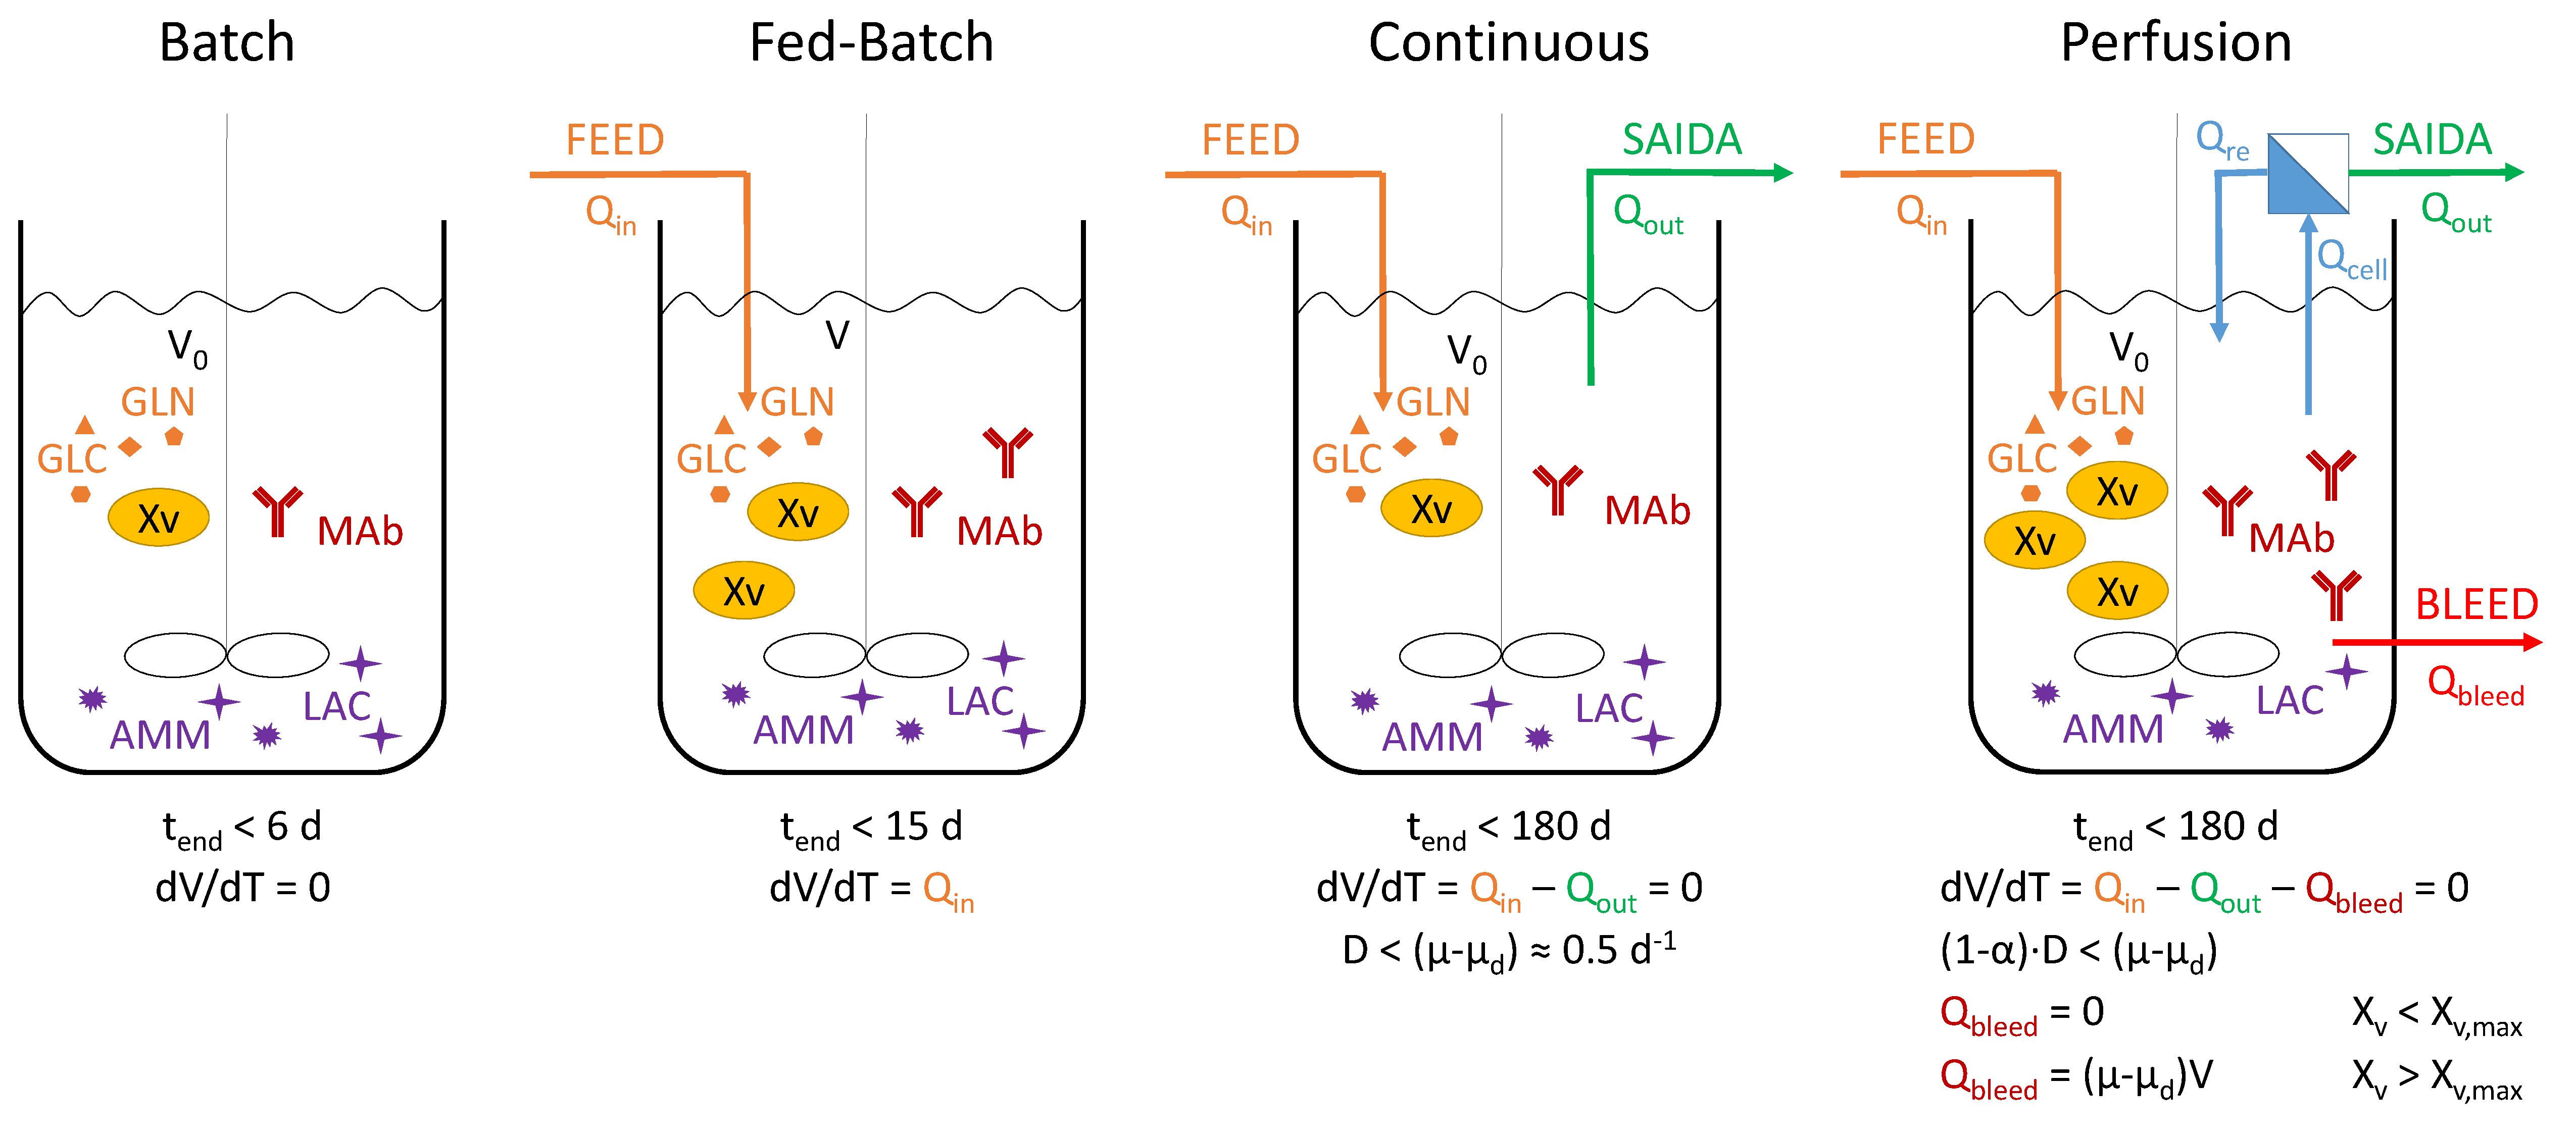
\includegraphics[width=\linewidth]{operation.pdf}
	\caption{Modos de operação de biorreatores de tanque agitado: Primeiro, a batelada simples, em que o tanque tem concentrações inicias de células e substrato. O tempo de operação $t_{end}$ é limitado pelo consumo dos substratos GLC e GLN e pela acumulação dos co-produtos tóxicos LAC e AMM. Na batelada alimentada, novos substratos são adicionados durante o processo, que aumenta máximo tempo de operação do biorreator para 15 dias. No modo de operação contínuo, um vazão de saída é adicionado e o volume mantido constante. A taxa de diluição $D$ do reator é limitado pela taxa de crescimento das células. Se for maior, mais células são retiradas do reator do que produzidas, um fenômeno chamado \textit{washout}. Na operação em perfusão, um reciclo de células é adicionado na vazão de saída. Assim são permitidos taxas de diluição altas sem levar ao \textit{washout} do biorreator, e concentrações altas de células são alcançadas. O tempo de operação ambos no continuo e na perfusão é limitado pelo fato que as células podem sofrer alterações genéticas durante o processo, que podem afeitar a qualidade do produto.}
	\label{fig:operation}
\end{figure*}

Nesse trabalho, os modos de operação de biorreatores em tanque agitado batelada simples, batelada alimentada, continuo simples, e perfusão foram modeladas e comparadas. A modelagem foi realizada a partir de um modelo da produção de anticorpos monoclonais (anti-TNP) com células hibridomas em modo de operação batelada simples, que foi validado com dados experimentais pelos autores \cite{Alves2008}.

Baseados nesses modelos, estudos de otimização dinâmica e controle preditivo foram realizados. Afinal, a possibilidade da integração da otimização dinâmica em tempo real (D-RTO) e do controle preditivo (MPC) foi discutido. 

%------------------------------------------------
\section{Modelagem}
A partir de um modelo da produção de anticorpos monoclonais (anti-TNP) com células hibridomas em modo de operação batelada simples \cite{Alves2008}, que foi validado com dados experimentais pelos autores, a modelagem dos modos de operação batelada alimentada, continuou e perfusão foi realizada. A figura \ref{fig:operation} destaca as principais diferenças entre os diferentes modos de operação.
\subsection{Batelada Simples}
O modelo do biorreator em modo de operação batelada simples foi adaptado de \cite{Alves2008}. Ele é constituído de duas equações algébricas (\ref{eq:algebric}), que descrevem a taxa de crescimento e morte das células, sete equações diferencias (\ref{eq:EDO}), que descrevem o balanço de massa de células, substratos e produtos no tempo, e 20 parâmetros (Tabela \ref{tab:parameters}). As taxas de crescimento $\mu$ e de morte $k_d$ especificas são baseados no modelo de Monod estendido, $\mu$ é limitado por glutamina (GLN) e inibido por amônio (AMM) e Lactato (LAC), e $k_d$ é inibido por GLN e limitado por AMM e LAC (Equações \ref{eq:algebrica} e \ref{eq:algebricb}).
A taxa de produção de células viáveis $\frac{dX_V}{dt}$ é expressa como diferença entre taxa de crescimento e taxa de morte das células (Equação \ref{eq:EDOa}). A taxa de consumo de glicose $\frac{dGLC}{dt}$ é divido em crescimento celular e formação de LAC (Equação \ref{eq:EDOc}). A taxa de consumo de glutamina $\frac{dGLN}{dt}$ consista da decomposição química de primeira ordem, da formação de células viáveis e da formação de AMM (Equação \ref{eq:EDOd}). As taxas $\frac{dLAC}{dt}$ e $\frac{dAMM}{dt}$ são associadas com o crescimento celular, e no caso do LAC também com a manutenção das células (Equações \ref{eq:EDOe} e \ref{eq:EDOf}). A taxa de produção do anticorpo monoclonal $\frac{dMAb}{dt}$ é parcialmente associado ao crescimento celular (Equação \ref{eq:EDOg}). As condições iniciais encontram-se na tabela \ref{tab:initial}.


\begin{figure}[ht]\centering
	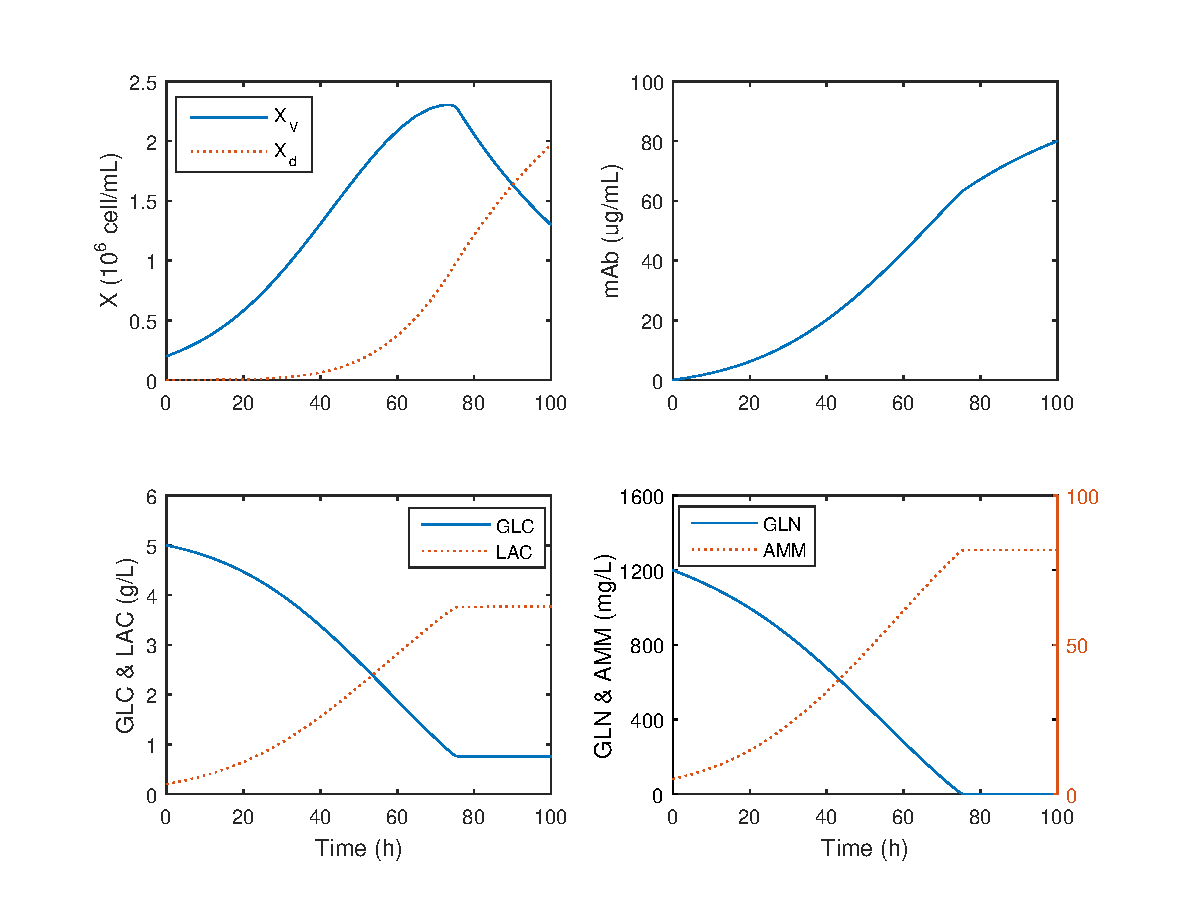
\includegraphics[width=\linewidth]{model1_validation}
	\caption{Validação do modelo da batelada simples.}
	\label{fig:model1_validation}
\end{figure}

\begin{subequations}  \label{eq:algebric}
\begin{multline} \label{eq:algebrica}
	\mu _X = \mu _{X,max}\left[\frac{GLN}{k_{GLN} + GLN}\right] \\ \left[\frac{k_{i,AMM}}{k_{i,AMM}+AMM}\right] \left[\frac{k_{i,LAC}}{k_{i,LAC} + LAC}\right]
\end{multline}
\begin{multline} \label{eq:algebricb}
	k_d=k_{d,max} \left[\frac{AMM}{k_{AMM}^d+AMM}\right] \\ \left[\frac{LAC}{k_{LAC}^d+LAC}\right] \left[\frac{k_{i,GLN}^d}{k_{i,GLN}^d + GLN}\right]
\end{multline}
\end{subequations}

\begin{subequations} \label{eq:EDO}
	\begin{align}
	&\frac{dX_V}{dt}\!\!\!\!\!\!\!\!\!\!&=& \;\, \mu _X X_V -k_d X_V \label{eq:EDOa}
	\\
	&\frac{dX_d}{dt}\!\!\!\!\!\!\!\!\!\!&=& \;\, k_d X_v \label{eq:EDOb}
	\\
	&\frac{dGLC}{dt}\!\!\!\!\!\!\!\!\!\!&=& \;\, -\frac{\mu _X X_v}{Y_{Xv/GLC}}-\frac{a_1 \mu _X X_v}{Y_{LAC/GLC}} \label{eq:EDOc}
	\\
	&\frac{dGLN}{dt}\!\!\!\!\!\!\!\!\!\!&=& \;\, -K.GLN -\frac{\mu _X X_v}{Y_{Xv/GLN}}-\frac{a_2 \mu _X X_v}{Y_{AMM/GLN}} \label{eq:EDOd}
	\\
	&\frac{dLAC}{dt}\!\!\!\!\!\!\!\!\!\!&=& \;\, a_3 \mu _X X_V + b_1 X_V \label{eq:EDOe}
	\\
	&\frac{dAMM}{dt}\!\!\!\!\!\!\!\!\!\!&=& \;\, a_4 \mu _X X_V \label{eq:EDOf}
	\\
	&\frac{dMAb}{dt}\!\!\!\!\!\!\!\!\!\!&=& \;\, a_5 \mu _X X_v+b_2 X_V \label{eq:EDOg}
	\end{align}	
\end{subequations}
Para validação, o modelo foi implementado em MATLAB R2015a e resolvido com o solver ode45. Os resultados são mostrados em Figura \ref{fig:model1_validation} e pode se observar a cinética comum de um bioprocesso em batelada simples, as células se duplicam exponencialmente até a depleção dos nutrientes (GLC e GLN). Durante da fase de crescimento acumulam-se os co-produtos LAC e AMM, que são inibidores do crescimento e promovem o morte das células. Porem, sem nutrientes e na presença de AMM e LAC em concentrações elevadas, começa a fase de morte das células. Com o morte das células a formação do produto MAb é limitado, e a batelada chega ao fim. Os gráficos obtidos são similares com os mostrados por \cite{Alves2008}, então o modelo pode ser considerado como válido.

\begin{table}
	\caption{Condições Iniciais}
	\centering
	\begin{tabular}{lcr}
		\toprule
		Variável & Unidade & Valor \\
		\midrule
		$X_V$ & \si{cells/L} & \num{0.2e9} \\
		$X_d$ & \si{cells/L} & \num{0} \\
		$GLC$ & \si{g/L} & \num{5} \\
		$GLN$ & \si{g/L} & \num{1.2} \\
		$LAC$ & \si{g/L} & \num{0.2} \\
		$AMM$ & \si{g/L} & \num{0} \\
		$MAb$ & \si{g/L} & \num{0} \\
		$V$ & \si{L} & \num{400} \\
	\end{tabular}
	\label{tab:initial}
\end{table}


\subsection{Batelada Alimentada}
Para evitar o problema da depleção de nutrientes, é comum operar o biorreator em batelada alimentada, em que uma vazão de entrada $Q_{in}$ suplementa o reator com meio novo. As equações \ref{eq:EDO2} mostram o modelo reformulado para a operação batelada alimentada. Como o volume não e mais constante mas suspeito à mudança pela vazão de entrada, foi adicionada a equação \ref{eq:EDO2h}. As outras equações, todas concentrações em função ao volume, foram modificadas em respeito à mudança do volume. Nas equações de GLC e GLN foram adicionados termos que respondem à adição de nutrientes, a vazão de entrada multiplicando com a concentração de GLC e GLN no meio de alimentação, $GLC_{in}$ e $GLN_{in}$ respectivamente.
\begin{subequations} \label{eq:EDO2}
	\begin{align}
	&\frac{d(VX_V)}{dt}\!\!\!\!\!\!\!\!\!\!&=& \;\, \left( \mu _X X_V -k_d X_V\right) V \label{eq:EDO2a}
	\\
	&\frac{d(VX_d)}{dt}\!\!\!\!\!\!\!\!\!\!&=& \;\, \left( k_d X_v\right) V \label{eq:EDO2b}
	\\
	&\frac{d(VGLC)}{dt}\!\!\!\!\!\!\!\!\!\!&=& \;\, \left( -\frac{\mu _X X_v}{Y_{Xv/GLC}}-\frac{a_1 \mu _X X_v}{Y_{LAC/GLC}} + Q_{in}GLC_{in}\right) V \label{eq:EDO2c}
	\\	&\frac{d(VGLN)}{dt}\!\!\!\!\!\!\!\!\!\!&=& \;\, \bigg(-K.GLN -\frac{\mu _X X_v}{Y_{Xv/GLN}} \label{eq:EDO2d} \\ & & & \;\, -\frac{a_2 \mu _X X_v}{Y_{AMM/GLN}}+ Q_{in}GLN_{in}\bigg)V \nonumber
	\\
	&\frac{d(VLAC)}{dt}\!\!\!\!\!\!\!\!\!\!&=& \;\, \left( a_3 \mu _X X_V + b_1 X_V\right) V \label{eq:EDO2e}
	\\
	&\frac{d(VAMM)}{dt}\!\!\!\!\!\!\!\!\!\!&=& \;\, \left( a_4 \mu _X X_V\right) V \label{eq:EDO2f}
	\\
	&\frac{d(VMAb)}{dt}\!\!\!\!\!\!\!\!\!\!&=& \;\, \left( a_5 \mu _X X_v+b_2 X_V\right) V \label{eq:EDO2g}
	\\
	&\frac{dV}{dt}\!\!\!\!\!\!\!\!\!\!&=& \;\, Q_{in} \label{eq:EDO2h}
	\end{align}	
\end{subequations}
Para não diluir o reator, o meio de alimentação costume ter concentrações elevadas das nutrientes. Aqui, foi escolhido um meio de alimentação cinco vezes mais concentrado que o meio de cultivo inicial. A alimentação pode ser feita seguindo diferentes estratégias, adição de nutrientes em impulsos, passos, escoamento constante ou controlado em respeito ao metabolismo das células. Na batelada alimentada, não só o tempo da operação aumenta, mas concentrações de células e produto maiores são alcançados. Na figura \ref{fig:model2} são mostrados os dados obtidos usando uma estratégia de alimentação comum, primeiro operar o biorreator sem alimentação, e quando os nutrientes chegam num nível baixo, ativar uma alimentação constante para fornecer novos nutrientes (aqui depois \SI{48}{h}).
\begin{figure}[ht]\centering
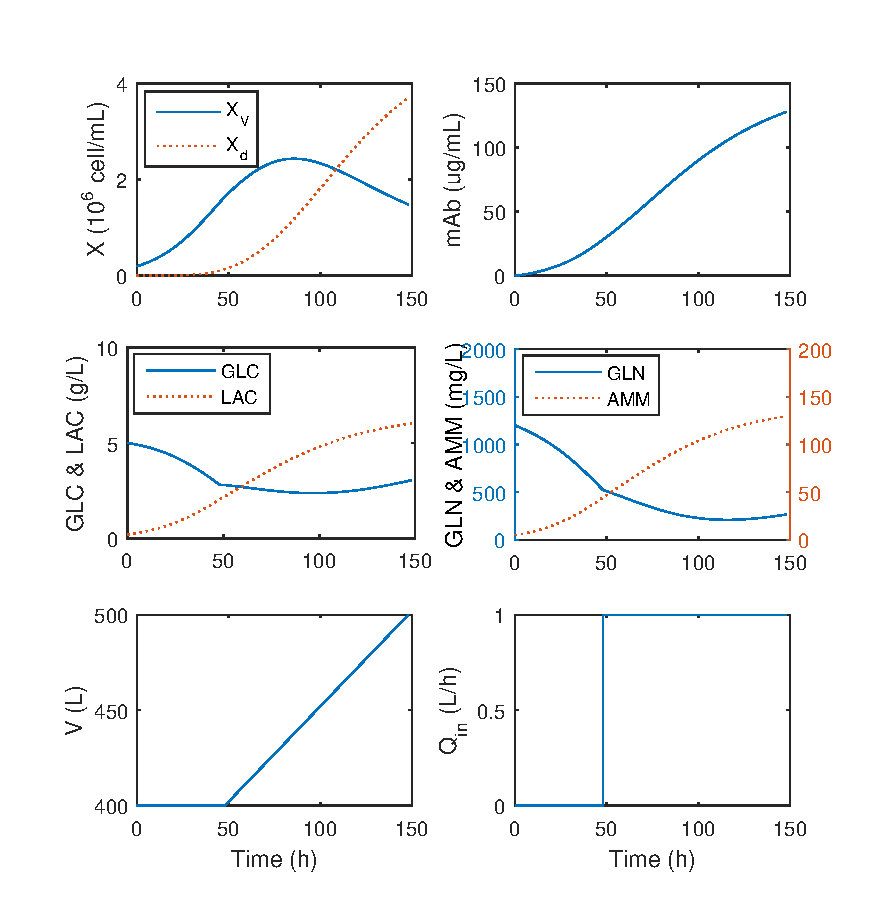
\includegraphics[width=\linewidth]{model2}
\caption{Operação em batelada alimentada.}
\label{fig:model2}
\end{figure}

Podemos observar um aumento no tempo de operação (\SI{148}{h} vs. \SI{100}{h} na batelada simples) e na concentração de produto final.

\subsection{Biorreator Contínuo} \label{continuo}

O biorreator continuo foi modelado a partir do modelo \ref{eq:EDO2} do biorreator em operação batelada alimentada. A equação diferencial para o volume foi acrescentado com o termo $-Q_{out}$, que representa o vazão de saída do reator:

\begin{equation}
	\frac{dV}{dt} = Q_{in} - Q_{out} \label{eq:Vcont}
\end{equation}

Os balanços de massa dos substratos, produtos e células com um termo do componente multiplicando $-Q_{out}$, que representa a taxa do componente retirado pelo vazão de saída. No seguinte, podemos acompanhar a transformação do modelo no exemplo do balanço de massa de células:

\begin{equation}
\frac{d(VX_V)}{dt} = \left( \mu _X X_V -k_d X_V \right) V -Q_{out}X_V\label{eq:Xvcont1}
\end{equation}
Agora, considerando que o volume é mantido constante durante o processo, ou seja, $Q_{in}$ = $Q_{out}$, obtemos: 

\begin{equation}
\frac{dV}{dt} = Q_{in} - Q_{out} = 0 \label{eq:Vcont0}
\end{equation}

Agora, dividindo a equação \ref{eq:Xvcont1} pelo volume, e introduzindo a diluição $D$ definido como vazão sobre volume $D = \frac{Q}{V}$ obtemos:

\begin{equation}
\frac{dX_V}{dt} = \mu _X X_V -k_d X_V -DX_V \label{eq:Xvcont2}
\end{equation}

Aplicando isso para todos balanços de massa obtemos o sistema:

\begin{subequations} \label{eq:EDO3}
	\begin{align}
	&\frac{dX_V}{dt}\!\!\!\!\!\!\!\!\!\!&=& \;\, \mu _X X_V -k_d X_V -DX_V \label{eq:EDO3a}
	\\
	&\frac{dX_d}{dt}\!\!\!\!\!\!\!\!\!\!&=& \;\, k_d X_v -DX_d\label{eq:EDO3b}
	\\
	&\frac{dGLC}{dt}\!\!\!\!\!\!\!\!\!\!&=& \;\, -\frac{\mu _X X_v}{Y_{Xv/GLC}}-\frac{a_1 \mu _X X_v}{Y_{LAC/GLC}} + D (GLC_{in} -GLC) \label{eq:EDO3c}
	\\	&\frac{dGLN}{dt}\!\!\!\!\!\!\!\!\!\!&=& \;\, -K.GLN -\frac{\mu _X X_v}{Y_{Xv/GLN}} \label{eq:EDO3d} \\ & & & \;\, -\frac{a_2 \mu _X X_v}{Y_{AMM/GLN}}+ D(GLN_{in} -GLN) \nonumber
	\\
	&\frac{dLAC}{dt}\!\!\!\!\!\!\!\!\!\!&=& \;\, a_3 \mu _X X_V + b_1 X_V -DLAC \label{eq:EDO3e}
	\\
	&\frac{dAMM}{dt}\!\!\!\!\!\!\!\!\!\!&=& \;\, a_4 \mu _X X_V -DAMM \label{eq:EDO3f}
	\\
	&\frac{dMAb}{dt}\!\!\!\!\!\!\!\!\!\!&=& \;\, a_5 \mu _X X_v+b_2 X_V -DMAb \label{eq:EDO3g}
	\end{align}	
\end{subequations}

No modo de operação continuo, a taxa de diluição é limitado pela taxa de crescimento das células. Se a taxa de diluição for maior que a taxa de proliferação $(\mu _X-k_d)$, o balanço de massa para $X_V$ vira negativa e a concentração cai, até possivelmente atingir um novo estado estacionário. Para uma diluição maior que a taxa especifica de crescimento celular máxima $\mu _{X,max}$, a concentração de células cai para 0, um processo chamado \textit{washout}. Porém, não é possível alcançar concentrações de células e produtividades elevadas, e o modo de operação continuo é mais usado para estudar o metabolismo das linhagens de células.

\begin{figure}[ht]\centering
	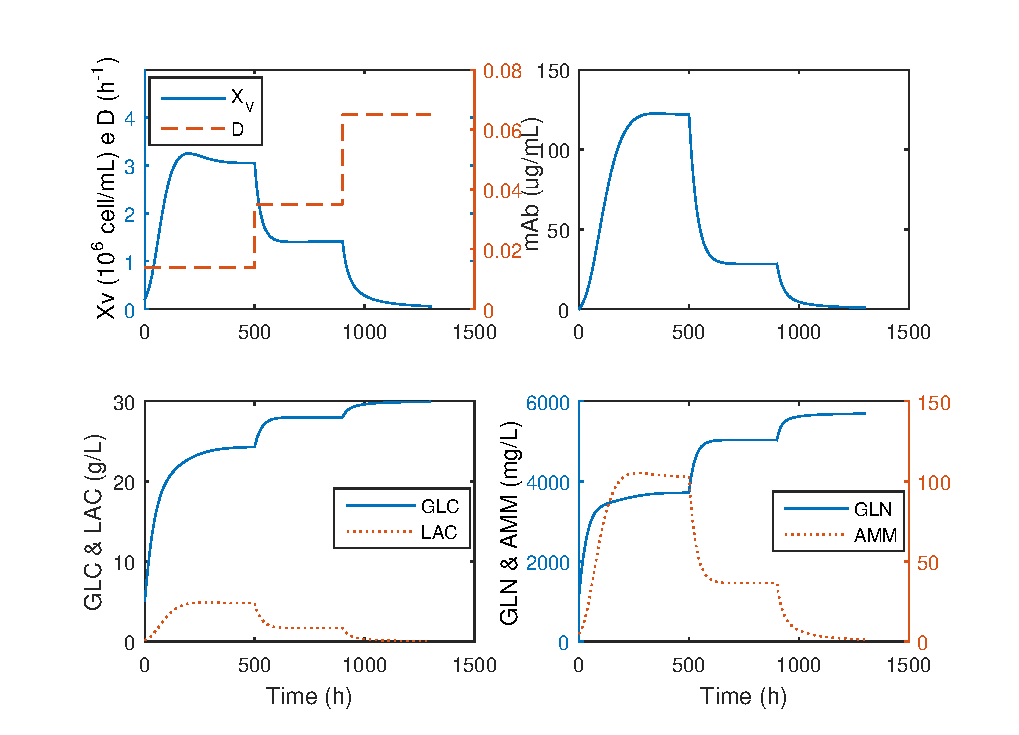
\includegraphics[width=\linewidth]{model3_d}
	\caption{Diferentes estados estacionários na operação continua, com taxas de diluição D diferentes.}
	\label{fig:model3_d}
\end{figure}

Na figura \ref{fig:model3_d} podemos ver o modelo com diferentes taxas de diluição, levando ao diferentes estados estacionários. Primeiro, uma taxa de diluição de \SI{0.0138}{\per\hour} leva a uma concentração de células elevada. Depois \SI{500}{\hour} a taxa de diluição é aumentado para \SI{0.035}{\per\hour}, e podemos observar um novo estado estacionário com concentrações de células e produtos menores e concentrações de substratos maiores. Com uma taxa de diluição \SI{0.065}{\per\hour}, um pouco maior que $\mu _{X,max}$ (\SI{0.063}{\per\hour}), vemos o efeito de \textit{washout}, as células são retiradas mais rápidos do que conseguem se proliferar, e logo a concentração cai para 0.

\begin{figure}[ht]\centering
	\includegraphics[width=\linewidth]{matcont}
	\setlength{\abovecaptionskip}{3pt}
	\caption{Continuação de equilíbrio do reator continuo}
	\label{fig:matcont}
\end{figure}

Para analisar os estados estacionários do sistema, continuação de equilíbrio (Figura \ref{fig:matcont}) foi feito com o pacote MatCont6p6 em MATLAB \cite{Dhooge2003}. Pode se observar os estados estacionários da concentração de células viáveis $X_V$ em função da diluição. Na diluição $D=\mu _{X,max}$, o estado do estacionário não há mais células (como esperado pelo \textit{washout}), e encontrou-se um ponto de bifurcação. A continuação do ponto de bifurcação revela que, sem células no reator, as concentrações do produtos são igual a \num{0} e a concentração de $GLC$ é igual a concentração de alimentação $GLC_{in}$. Apenas concentração de $GLN$ varia, que é explicado pela decomposição de primeira ordem da glutamina. Assim achou-se um erro no modelo, pois um dos produtos da decomposição de glutamina é a amônia, e isso não é representado pelas equações do modelo.

\subsection{Perfusão} \label{perfusion}
\begin{figure}[ht]\centering
	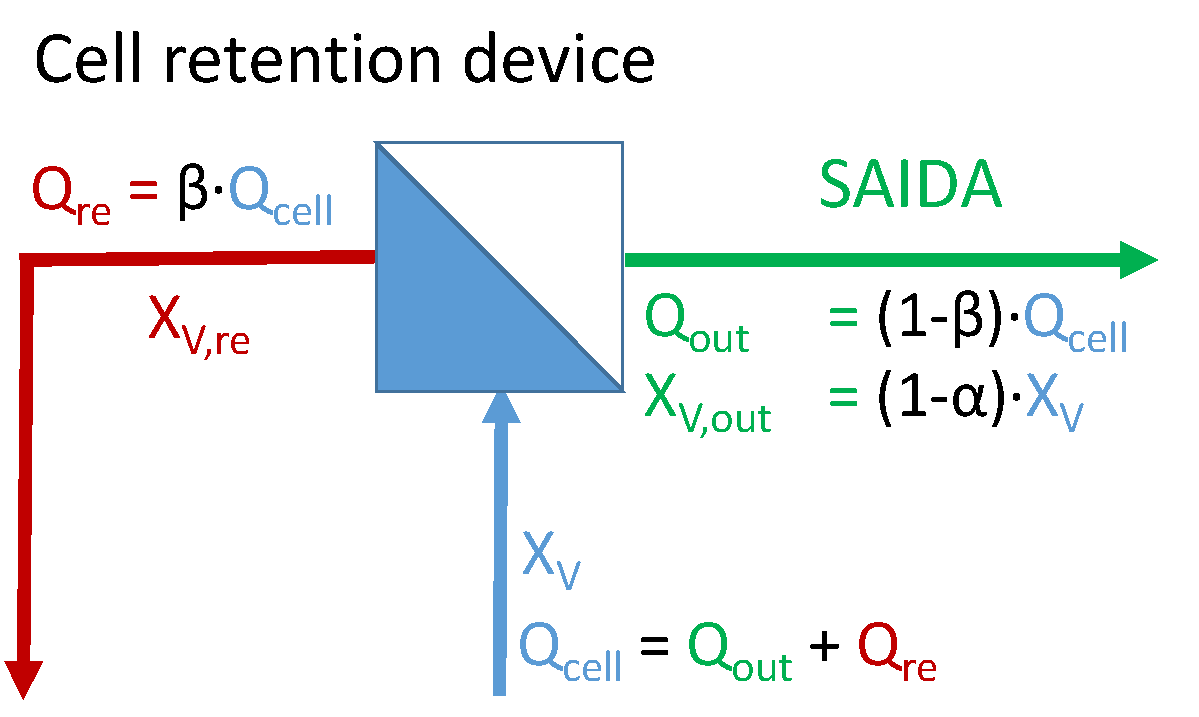
\includegraphics[width=\linewidth]{cellretention}
	\caption{Equipamento de retenção de células}
	\label{fig:cellretention}
\end{figure}

A modelagem do biorreator em perfusão foi feita a partir do modelo continuo \ref{eq:EDO3}. Na perfusão a vazão de saída é equipado com um equipamento de retenção de células, que separa com uma eficiência $\alpha$ as células e realimenta-as com o vazão de reciclo $Q_{re}$ no biorreator \ref{fig:cellretention}. Assim é superado o problema de \textit{Wash-Out} que limita a diluição na operação continua (Seção~\ref{continuo}), e com taxas de diluição altas, concentrações de células elevadas são alcançadas. Portanto, a concentração de células é limitada pela oxigenação do reator, pois é preciso controlar-a com \textit{cell bleeding}. Isso é a implementação de um vazão de \textit{bleeding} $Q_b$, que retira volume do reator sem retenção de células. Então a equação para o volume fica:
\begin{equation}
\frac{dV}{dt} = Q_{in} - Q_{out} - Q_b \label{eq:Vperf}
\end{equation}
 A vazão $Q_b$ é controlada para manter a concentração de células num nível constante. Controlando as vazões $Q_{in}$ e $Q_{out}$, o volume pode ser mantido constante, então foi considerado novamente $\frac{dV}{dt} = 0$.
 
Para os balanços de massa no equipamento de retenção de células:
\begin{align}
	Q_{cell} =&\; Q_{out} - Q_{re} \\
	Q_{cell}X_V =&\; Q_{out}X_{V,out} - Q_{re}X_{V,re}
\end{align}
Considerando a razão entre os vazões $\beta = \frac{Q_{re}}{Q_{cell}}$ no equipamento, com $0<\beta<1$ obtemos:
\begin{align}
Q_{re} =&\; \frac{\beta Q_{out}}{(1-\beta)} \\
Q_{cell}=&\; \frac{Q_{out}}{(1-\beta)}
\end{align}
E sabendo que $X_{V,out} = (1-\alpha)X_V$, obtemos com
\begin{equation}
	X_{V,re} = \frac{Q_{cell}X_V - Q_{out}(1-\alpha)X_V}{Q_{re}}
\end{equation}
tudo para escrever os novos balanços de massa para as células:
\begin{align}  \label{eq:EDO4cell}
\frac{dX_V}{dt} =&\;(\mu _X -k_d) X_V - Q_{cell}X_V + Q_{re}X_{V,re} - Q_b X_V
\end{align}
As mesmas mudanças aplicam-se para o balanço das células não viáveis $X_d$, pois o equipamento de retenção de células não distinta entre células viáveis e não viáveis. Assumindo uma eficiência $\alpha$ de 1, que é alcançado por modernos hidrociclones \cite{elsayed2006}, e pelo fato que $\frac{dV}{dt} = 0$, chegamos no sistema de balanços simplificado:
\begin{subequations} \label{eq:EDO4}
	\begin{align}
	&\frac{dX_V}{dt}\!\!\!\!\!\!\!\!\!\!&=& \;\, \mu _X X_V -k_d X_V -\frac{Q_b}{V}X_V \label{eq:EDO4a}
	\\
	&\frac{dX_d}{dt}\!\!\!\!\!\!\!\!\!\!&=& \;\, k_d X_v -\frac{Q_b}{V}X_d\label{eq:EDO4b}
	\\
	&\frac{dGLC}{dt}\!\!\!\!\!\!\!\!\!\!&=& \;\, -\frac{\mu _X X_v}{Y_{Xv/GLC}}-\frac{a_1 \mu _X X_v}{Y_{LAC/GLC}} + D (GLC_{in} -GLC) \label{eq:EDO4c}
	\\	&\frac{dGLN}{dt}\!\!\!\!\!\!\!\!\!\!&=& \;\, -K.GLN -\frac{\mu _X X_v}{Y_{Xv/GLN}} \label{eq:EDO4d} \\ & & & \;\, -\frac{a_2 \mu _X X_v}{Y_{AMM/GLN}}+ D(GLN_{in} -GLN) \nonumber
	\\
	&\frac{dLAC}{dt}\!\!\!\!\!\!\!\!\!\!&=& \;\, a_3 \mu _X X_V + b_1 X_V -DLAC \label{eq:EDO4e}
	\\
	&\frac{dAMM}{dt}\!\!\!\!\!\!\!\!\!\!&=& \;\, a_4 \mu _X X_V -DAMM \label{eq:EDO4f}
	\\
	&\frac{dMAb}{dt}\!\!\!\!\!\!\!\!\!\!&=& \;\, a_5 \mu _X X_v+b_2 X_V -DMAb \label{eq:EDO4g}
	\end{align}	
\end{subequations}
sendo a diluição D a razão entre $\frac{Q_{in}}{V}$. Para limitar a concentra-ção de células abaixo de um valor critico para a oxigenação, $X_{V,max}$, a vazão de \textit{bleeding} foi definido como:
\begin{equation}
Q_b =
	\begin{cases}
	0		& \quad \text{para } X_V < X_{V,max} \\
	(\mu _X - k_d)V & \quad \text{para } X_V > X_{V,max} \\
	\end{cases}
\end{equation}
Assim, para valores de $X_V$ maior que $X_{V,max}$, o balanço de massa das células $\frac{dX_V}{dt}$ é zerado, ou seja, o vazão $Q_b$ tira células do reator na mesma taxa de proliferação. Isso leva para os resultados desejados na simulação, porém, pelo fato que não é possível medir $(\mu _X - k_d)$ precisamente, não é aplicável na prática. São usados sensores de capacitância para medir $X_V$ \textit{on line} ou o oxigênio dissolvido como referência para o controle do processo \cite{Justice2011}.

\begin{figure}[ht]\centering
	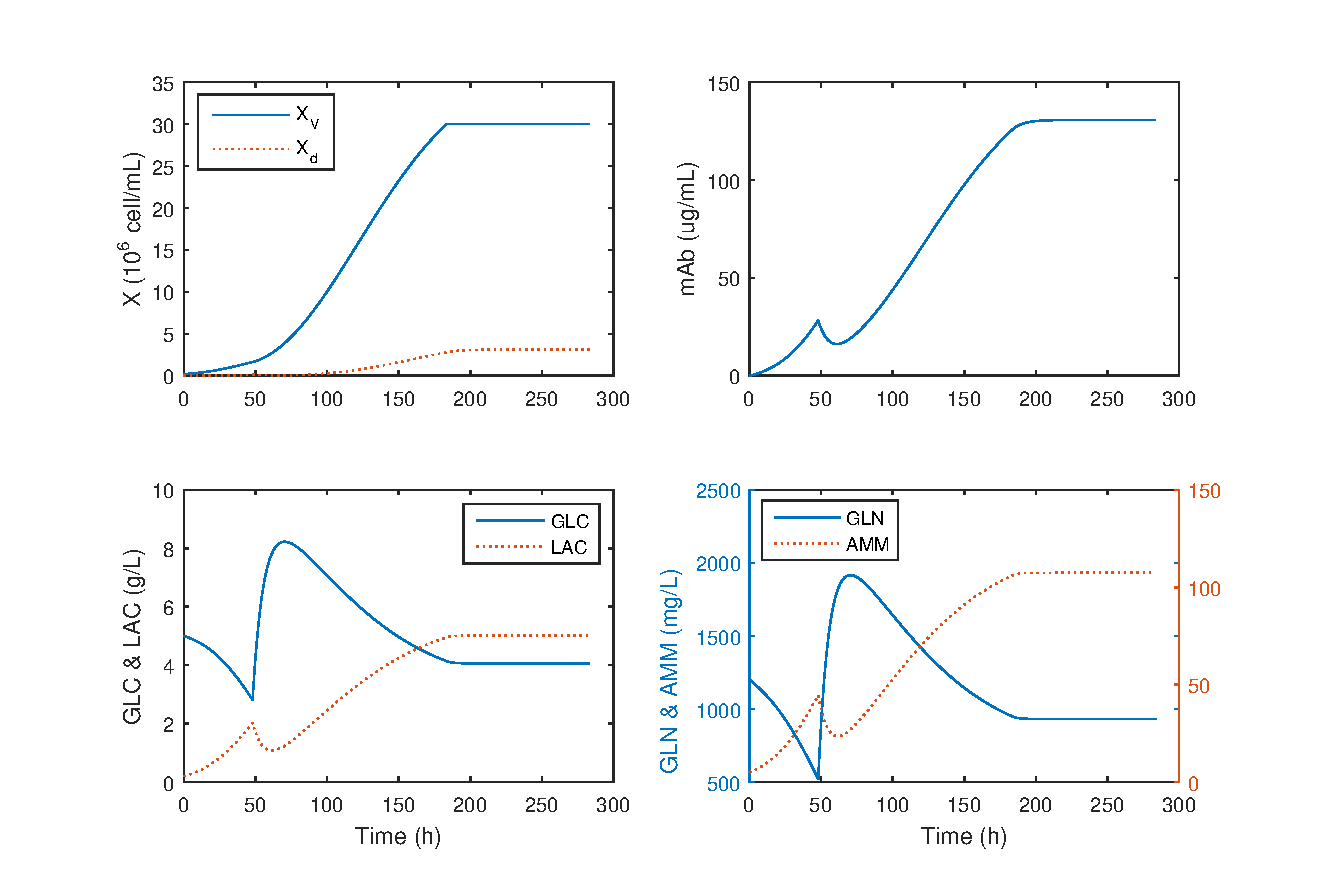
\includegraphics[width=\linewidth]{model4}
	\caption{Biorreator em perfusão}
	\label{fig:model4}
\end{figure}

A operação tipico de um reator em perfusão é mostrado na figura \ref{fig:model4}. A concentração do meio de alimentação foi escolhido duas vezes mais concentrado que o meio inicial da cultura, $GLC_{in} = \SI{10}{\g\per\L}$ e $GLN_{in} = \SI{2.4}{\g\per\L}$, respectivamente. Em t =  \SI{48}{\hour} uma diluição de \SI{3}{\per\day} é ligado e mantido constante. Os efeitos são o aumento de $GLC$ e $GLN$ e a retiração de $LAC$, $AMM$ e $mAB$ do reator. Pelo equipamento de retenção de células, a concentração de células não e afeitada, não há \textit{washout}. Assim, a concentração de células aumenta ilimitada até chegar perto da limitação de oxigênio, quando o \textit{bleeding} é ativada que controla a concentração de células num estado estacionário forçado (\SI{30e6}{cells\per\mL}).

\section{Otimização}

A otimização dinâmica foi realizada usando o pacote \textit{DYNOPT~4.3.0} em MATLAB~R2015a, que usa os métodos de colocação ortogonal e elementos finitas para transformar as problemas de otimização originais em problemas de programa-ção não-linear (NLP), que são resolvidos por solvers de NLP apropriados \cite{Cizniar2005}.

Nas seguintes seções, distintas estratégias da otimização são aplicados nos diferentes modos de operação. 

\subsection{Batelada simples}

Uma estratégia importante na otimização do modo de operação da batelada simples é a otimização do meio de cultivo. Porém, esses estudos tem que ser feito primeiramente empírico, pois os parâmetros dos modelos são sensíveis a mudanças no meio de cultivo.

\subsection{Batelada alimentada}

A otimização dinâmica foi usada para encontrar a melhor estratégia de alimentação na batelada alimentada. Como função objetivo foi considerado a concentração de anticorpo monoclonal no final da batelada, a vazão de entrada foi usado como variável de controle.
Assim, foi formulado o problema de otimização \ref{eq:otim}. As restrições incluem que a vazão de entrada não pode ser negativa, ou seja, só alimentação é permitida, e que o volume não pode ultrapassar \SI{500}{\liter}, para evitar diluição do biorreator.

\begin{equation} \label{eq:otim}
\begin{array}{rrclcl}
\displaystyle \max_{Q_{in}(t)} & \multicolumn{3}{l}{\Phi = MAb(t_f)} \\
& & & \\
\textrm{sujeito a} & Q_{in}(t) & \geq & \SI[per-mode=fraction]{0}{\liter\per\hour} \\
& V (t)& \leq & \SI{500}{\liter}\\
\end{array}
\end{equation}

Na figura \ref{fig:model2_ncolu1} encontra-se os resultados da otimização com uma colocação da variável manipulada $Q_{in}(t)$ em 4 elementos finitos. O ótimo encontrado foi de $MAb(t_f) = \SI{147,602}{ \mg\per\L}$. Com duas colocações, o ótimo encontrado foi de $MAb(t_f) = \SI{150,665}{ \mg\per\L}$ (gráfico não mostrado). 

\begin{figure}[ht]\centering
	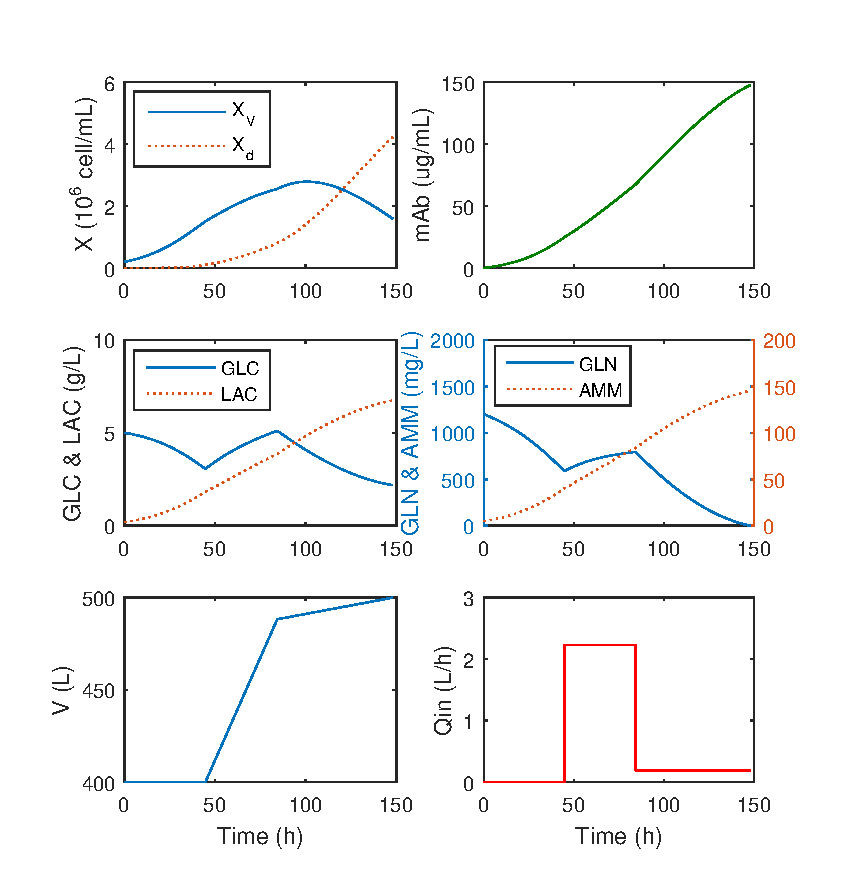
\includegraphics[width=\linewidth]{model2_ncolu1}
	\caption{Batelada alimentada otimizada}
	\label{fig:model2_ncolu1}
\end{figure}

\subsection{Biorreator Continuo}

Na operação continua, foi primeiro determinada qual o estado estacionário com a maior produtividade volumétrica de anticorpos $Q_{MAb} = D MAb$. O problema de otimização foi formulado como:

\begin{equation} \label{eq:otim2}
\begin{array}{rrclcl}
\displaystyle \max_{D} & \multicolumn{3}{l}{\Phi = Q_{MAb}} \\
& & & \\
\textrm{sujeito a} & D & \geq & \SI{0}{\per\hour} \\
\end{array}
\end{equation}
O ótimo encontrado é de $Q_{MAb} = \SI{1,6838}{\mg\per\liter\per\hour}$, para uma taxa de diluição $D = \SI{0.0138}{\per\hour}$ e uma concentração de células $X_V = \SI{3.06e6}{cells \per\mL}$. Porém, nesta taxa de diluição o estado estacionário é apenas atingido depois aproximadamente \SI{400}{\hour}, como pode se verificar na figura \ref{continuo}. Para aproveitar uma outra possibilidade da optimização dinâmica, foi escolhido melhorar o tempo até chegar na concentração de células do estado estacionário. O problema de otimização foi formulado:

\begin{equation} \label{eq:otim3}
\begin{array}{rrclcl}
\displaystyle \min_{D(t)} & \multicolumn{3}{l}{\Phi = t_{f}} \\
& & & \\
\textrm{sujeito a} & X_V(t_{f}) & = & \SI{3.06e6}{cells \per\mL} \\
& D & \geq & \SI{0}{\per\hour}\\
\end{array}
\end{equation}
O tempo minimo encontrado foi de $t_{f} = \SI{84,8977}{\hour}$ para uma colocação de D e de $t_{f} = \SI{84,7459}{\hour}$ para duas colocações em D (Figura \ref{fig:model3_ncolu2}). Esses tempos não representam o tempo necessário até chegar no estado estacionário, para isso precisaria ser implementado restrições dizendo que as derivadas de todas as variáveis são nulas em $t_{f}$.

\begin{figure}[ht]\centering
	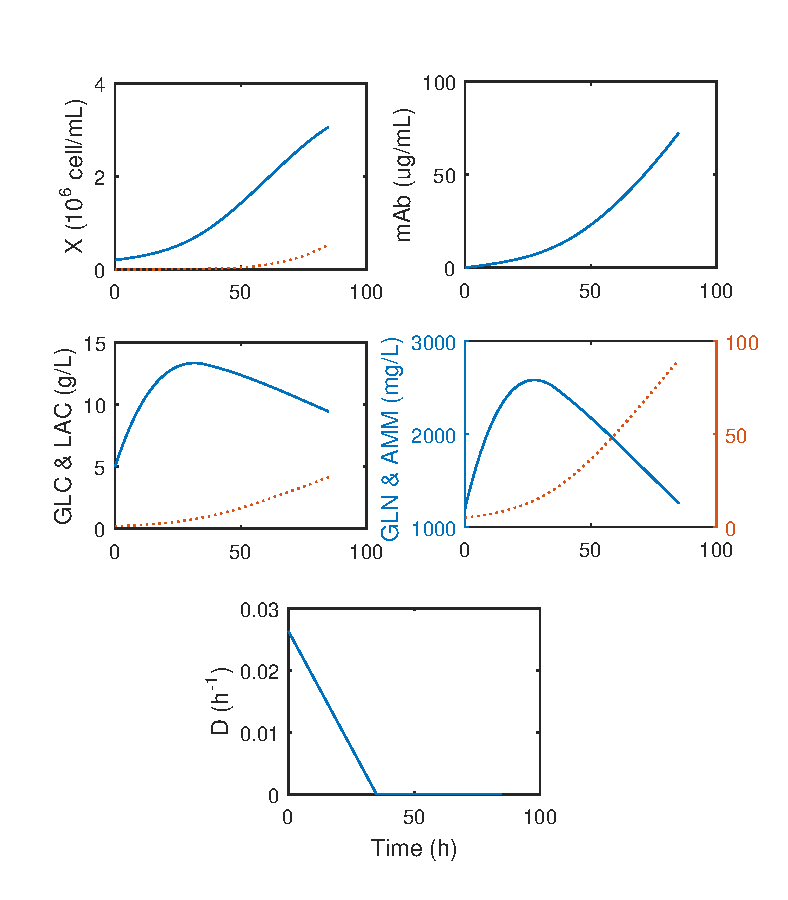
\includegraphics[width=\linewidth]{model3_ncolu2}
	\caption{Perfil de diluição com duas colocações em D}
	\label{fig:model3_ncolu2}
\end{figure}

O tempo minimo também foi determinado para uma taxa de diluição constante, com  \textit{fmincon} (algoritmo ponto-interior) em MATLAB, usando a opção \textit{event} para terminar a integração ao chegar em $X_V = \SI{3.06e6}{cells \per\mL}$. O ótimo encontrado foi de $t_{f} = \SI{98,2853}{\hour}$, para uma taxa de diluição de \SI{0.0051}{\per\day}.
Isto é, \SI{16}{\%} maior comparado com os resultados da otimização dinâmica. 
\subsection{Perfusão}

A perfusão é o modo de operação mais complicado, e um desafio é o controle da concentração de células, como foi discutido na secção \ref{perfusion}. Então foi escolhido como objetivo melhorar o controle por volta do estado estacionário. O processo foi identificado (linearização no estado estacionário de \SI{30e6}{cells \per\mL}) e um controlador preditivo (MPC) criado usando o MPCTOOL em MATLAB/SIMULINK. Como pertubações possíveis foram escolhidos mudanças no meio de alimentação. O processo todo foi incluso em SIMULINK é testado dando pertubações na entrada e dando um novo setpoint para $X_V$ (Figura \ref{fig:MPC2}). 

\begin{figure}[ht]\centering
	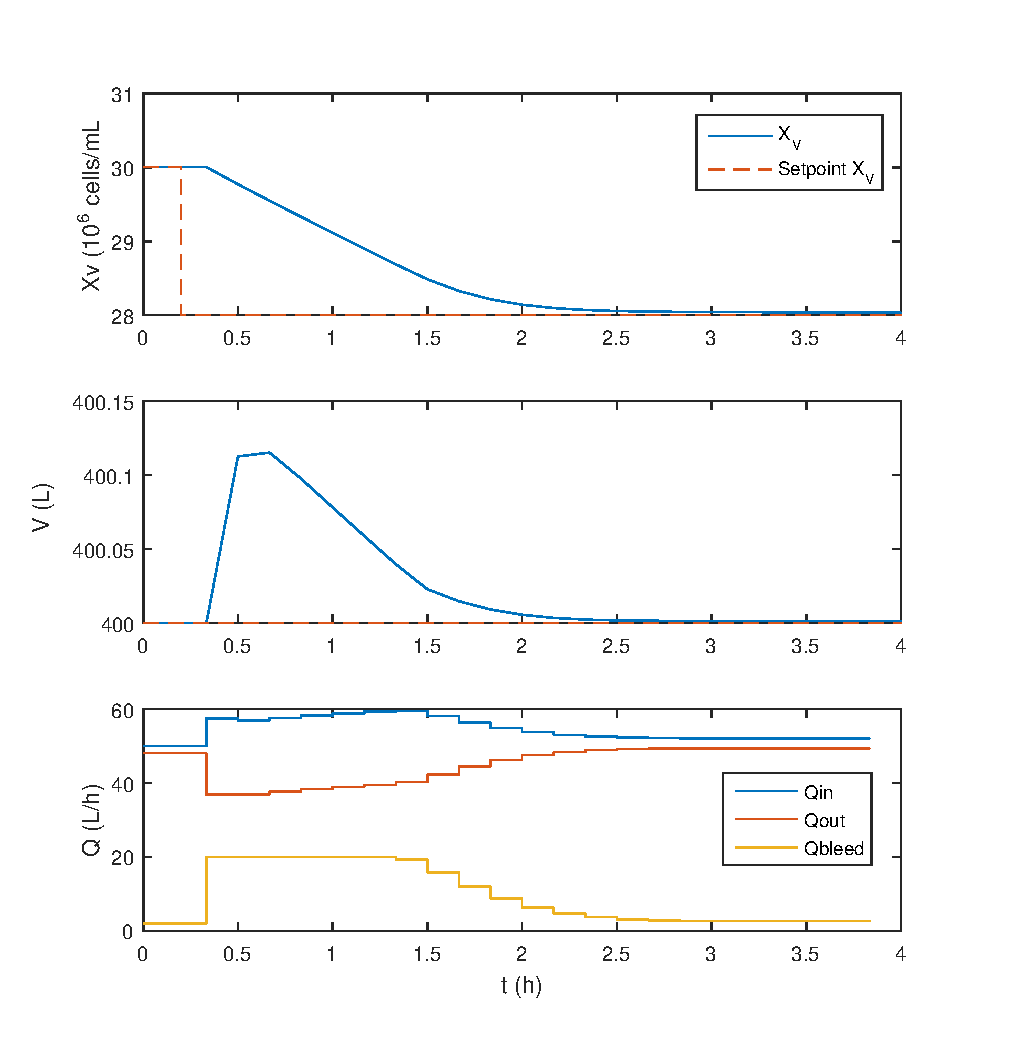
\includegraphics[width=\linewidth]{MPC2}
	\caption{MPC atuando em intervalos de \SI{10}{\minute} para levar $X_V$ de 30 para um novo setpoint de \SI{28e6}{cells \per\mL.}}
	\label{fig:MPC2}
\end{figure}

O resultado foi comparado com a trajetória do tempo minimo por DYNOPT. O problema de otimização foi formulado como:

\begin{equation} \label{eq:otim4}
\begin{array}{rrclcl}
\displaystyle \min_{Q(t)} & \multicolumn{3}{l}{\Phi = t_{f}} \\
& & & \\
\textrm{sujeito a} &&& X_V(t_{f}) & = & \SI{28e6}{cells \per\mL} \\
& \SI{0}{ \L\per\hour} & \leq & Q_{in}(t) & \leq &\SI{100}{ \L\per\hour}\\
& \SI{0}{ \L\per\hour} & \leq & Q_{out}(t) & \leq&\SI{100}{ \L\per\hour}\\
& \SI{0}{ \L\per\hour} & \leq & Q_{b}(t) & \leq &\SI{20}{ \L\per\hour}\\
& \SI{390}{ \L} & \leq & V(t) & \leq &\SI{410}{ \L}
\end{array}
\end{equation}

As restrições são as mesmas que foram dados para o MPC. O minimo encontrado é de $t_{f} = \SI{1.4716}{\hour}$, e os resultados são encontrados em figura \ref{fig:model4tmin}. A resposta ambos da optimização e do MPC para levar a concentração de células para \SI{28e6}{cells \per\mL} é de aumentar o vazão de \textit{bleeding} $Q_b$ para o máximo da restrição. O resultado da otimização dinâmica indica que o caminho mais rápido é de manter $Q_{out}$ no minimo de \SI{0}{ \L\per\hour}, mas essa solução não garanta estabilidade no final. Foi tentado implementar a otimização dinâmica como \textit{dynamic real time optimization} (D-RTO) para dar uma trajetória de setpoints ótimos para o MPC operar, mas a implementação falhou por causa de incompletabilidades entre algumas funções do DynOpt e a compilação de Simulink.

\begin{figure}[ht]\centering
	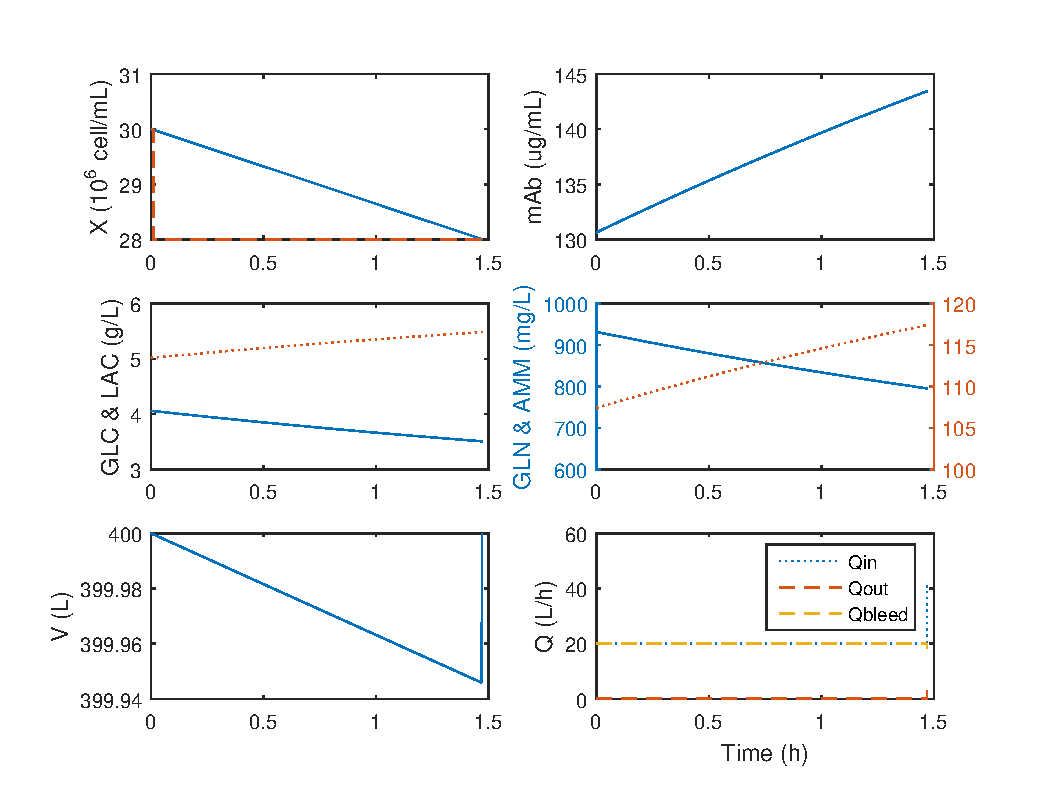
\includegraphics[width=\linewidth]{model4_tmin3}
	\caption{Resultado da otimização dinâmica}
	\label{fig:model4tmin}
\end{figure}
%------------------------------------------------

\section{Resultados e Discussão}

\begin{table}
	\caption{Comparação - modos de operação}
	\centering
	\begin{tabular}{lr}
		\toprule
		Operação & Produtividade\\
		\midrule	
		Batelada simples & \SI{19.217}{ \mg\per\L\per\day}\\
		Batelada alimentada & \SI{25.928}{ \mg\per\L\per\day}\\
		Batelada alimentada otimizada & \SI{30.540}{ \mg\per\L\per\day}\\
		Continua & \SI{1.683}{ \mg\per\L\per\day}\\
		Perfusão & \SI{391.886}{ \mg\per\L\per\day}
	\end{tabular}
	\label{tab:results}
\end{table}

Nas secções anteriores, os diferentes modos de operação de biorreatores em tanque agitado foram apresentados, modelados, e optimizados. Na tabela \ref{tab:results} os resultados dos diferentes modos de operação são comparadas. Os cálculos para os processos em batelada foram feitos sem considerar o tempo entre cada batelada necessário para limpeza e esterilização do biorreator. Os dados destacam claramente a perfusão como modo de operação superior, com uma produtividade volumétrica mais que 10 vezes maior que da batelada alimentada otimizada. Pensando na escala do processo de produção, o processo em perfusão ia permitir uma planta de produção muito menor para a mesma quantidade de produto. Porém, na industria o processo de perfusão ainda não é muito estabelecido. Isto tem por causa a grande complexabilidade em comparação com os processos em batelada alimentada, que são os mais usados para produção de biofármacos.

Podemos concluir que as disciplinas de otimização e controle, ambos baseados em modelos robustos, oferecem grandes possibilidades para a industria biofarmacêutica, que é hoje em dia principalmente baseado em estudos empíricos.



\begin{table*}[hb]
	\caption{Tabela de parâmetros}
	\centering
	\begin{tabular}{lllr}
		\toprule
		Parâmetro & Descrição & Unidade & Valor\\
		\midrule
		$\mu _{X,max}$ & Taxa especifica de crescimento celular máxima & $h^{-1}$ & 6.30 $\cdot$ 10\textsuperscript{-2}\\
		$k_{GLN}$ & Constante de limitação da glutamina para crescimento & $g/L$ & 2.65 $\cdot$ 10\textsuperscript{-3}\\
		$k_{i,AMM}$ & Constante de inibição do amônio para crescimento & $g/L$ & 6.57 $\cdot$ 10\textsuperscript{-2}\\
		$k_{i,LAC}$ & Constante de inibição do lactato para crescimento & $ g/L $ & 15.1\\
		$k_{d,max}$ & Taxa especifica de morte celular máxima & $h^{-1}$ & 7.63 $\cdot$ 10\textsuperscript{-2}\\
		$k_{AMM}^d$ & Constante de limitação do amônio para morte& $ g/L $ & 2.19 $\cdot$ 10\textsuperscript{-2}\\
		$k_{LAC}^d$ & Constante de limitação do lactato para morte& $ g/L $ & 6.11\\
		$k_{i,GLN}^d$ & Constante de inibição da glutamina para morte& $ g/L $ & 0.778\\
		$Y_{X_v/GLC}$ & Constante de rendimento glicose para células viáveis & $cells/g$ &  1.16 $\cdot$ 10\textsuperscript{9}\\
		$Y_{LAC/GLC}$ & Constante de rendimento glicose para lactato & $ g/g $ & 1.00\\
		$Y_{X_v/GLN}$ & Constante de rendimento glutamina para células viáveis& $ cells/g $ & 2.09 $\cdot$ 10\textsuperscript{10}\\
		$Y_{AMM/GLN}$ & Constante de rendimento glutamina para amônio & $g/g$ & 2.10 $\cdot$ 10\textsuperscript{2}\\
		$K$ & Constante de primeira ordem para decomposição de glutamina & $h^{-1}$ &3.34 $\cdot$ 10\textsuperscript{-3}\\
		$a_1$ & Constante para consumo de glicose associada ao crescimento& $ g/cell $ &5.20 $\cdot$ 10\textsuperscript{8}\\
		$a_2$ & Constante para consumo de glutamina associada ao crescimento& $ g/cell $ & 7.05 $\cdot$ 10\textsuperscript{12}\\
		$a_3$ & Constante para formação de lactato associada ao crescimento& $ g/cell $ &  1.15 $\cdot$ 10\textsuperscript{9}\\
		$a_4$ & Constante para formação de amônio  associada ao crescimento & $ g/cell $ & 2.5 $\cdot$ 10\textsuperscript{11}\\
		$a_5$ & Constante para formação de MAb associada ao crescimento  & $ g/cell $  & 8.67 $\cdot$ 10\textsuperscript{9}\\
		$b_1$ & Constante para formação de lactato não associada ao crescimento & $ g/(cell\cdot h) $ & 3.12 $\cdot$ 10\textsuperscript{10}\\
		$b_2$ & Constante para formação de MAb não associada ao crescimento & $ g/(cell\cdot h) $ & 3.89 $\cdot$ 10\textsuperscript{10}\\
	\end{tabular}
	\label{tab:parameters}
\end{table*}


%------------------------------------------------
\phantomsection
\section*{Agradecimentos} % The \section*{} command stops section numbering
Agradeço ao Leonardo do Laboratório de Desenvolvimento de Software para Otimização e Controle de Processos (Lades, COPPE/UFRJ), pelo suporte no conceito e na implementação do MPC + D-RTO.

\addcontentsline{toc}{section}{Agradecimentos} % Adds this section to the table of contents

%----------------------------------------------------------------------------------------
%	REFERENCE LIST
%----------------------------------------------------------------------------------------
\phantomsection
\bibliographystyle{unsrtnat}		% definir o estilo da bibliografia com o pacote natbib
\bibliography{optimization} 		% definir o arquivo para bibtex

%----------------------------------------------------------------------------------------
\end{document}